\documentclass[25pt,a0paper,portrait,margin=0mm,innermargin=15mm,blockverticalspace=12mm,colspace=12mm]{tikzposter}
\usepackage{graphicx,booktabs,qrcode}
\graphicspath{{../docs/img/}}
% Generated by  python -m adamas.paper  from the ADAMAS package. Do not edit by hand.
\newcommand{\BFOMratio}{48{,}976}
\newcommand{\KappaRatio}{14.7}
\newcommand{\MeasuredOverSi}{89}
\newcommand{\BestBV}{3659}
\newcommand{\LossSi}{209.5}
\newcommand{\LossSiC}{29.7}
\newcommand{\LossGaN}{20.6}
\newcommand{\LossDiamond}{3.8}
\newcommand{\LossDiamondMeasured}{89}
\newcommand{\GateTimeUs}{25}
\newcommand{\FcohPublished}{0.998}
\newcommand{\qForSixtySeven}{0.75}
\newcommand{\qForEightyTwo}{0.87}
\newcommand{\ReadoutContrast}{45}
\newcommand{\Polarization}{82}
\newcommand{\LambdaFast}{4.03}
\newcommand{\LambdaMs}{3.56}
\newcommand{\LambdaTenMs}{2.64}
\newcommand{\RSADistance}{57}
\newcommand{\RSAQubitsM}{78}
\newcommand{\RSADieMm}{5.7}
\newcommand{\RSAYears}{6.0}
\newcommand{\RSAYearsFast}{1.0}
\newcommand{\RSADaysSC}{4}
\newcommand{\DiaCells}{323}
\newcommand{\NumRefs}{541}
\newcommand{\NumVerified}{500}
\newcommand{\NumFigures}{52}
\newcommand{\UncPowerPten}{2.5}
\newcommand{\UncPowerPfifty}{3.8}
\newcommand{\UncPowerPninety}{5.5}
\newcommand{\UncQPten}{1.2}
\newcommand{\UncQPfifty}{3.6}
\newcommand{\UncQPninety}{15.5}
\newcommand{\ValChecks}{19}
\newcommand{\ValPass}{18}
\newcommand{\ThrCSSBias}{0.63}
\newcommand{\ThrXZZXBias}{1.59}
\newcommand{\ThrDepol}{0.95}
\newcommand{\NativeGain}{12}
\newcommand{\RSADistanceCSSBiased}{129}
\newcommand{\RSAQubitsMCSSBiased}{399}
\newcommand{\RSAYearsCSSBiased}{13.6}
\newcommand{\RSADistanceXZZX}{53}
\newcommand{\RSAQubitsMXZZX}{67}
\newcommand{\RSAYearsXZZX}{5.6}
\newcommand{\SobolMobility}{0.42}
\newcommand{\SobolField}{0.42}
\newcommand{\SobolReadout}{0.96}
\newcommand{\XZZXDepolQubitsM}{142}
\newcommand{\CSSDepolQubitsM}{165}
\newcommand{\BreakevenStdMs}{100}
\newcommand{\BreakevenXZZXMs}{1000}

\definecolor{ink}{HTML}{1D2733}\definecolor{teal}{HTML}{0FA3B1}\definecolor{coral}{HTML}{E63946}\definecolor{paper}{HTML}{F5F8FA}
\definecolorstyle{adamas}{\definecolor{colorOne}{named}{ink}\definecolor{colorTwo}{named}{teal}\definecolor{colorThree}{named}{coral}}{
 \colorlet{backgroundcolor}{paper}\colorlet{framecolor}{ink}\colorlet{titlefgcolor}{white}\colorlet{titlebgcolor}{ink}
 \colorlet{blocktitlebgcolor}{teal}\colorlet{blocktitlefgcolor}{white}\colorlet{blockbodybgcolor}{white}\colorlet{blockbodyfgcolor}{ink}
 \colorlet{innerblocktitlebgcolor}{ink}\colorlet{innerblocktitlefgcolor}{white}\colorlet{innerblockbodybgcolor}{paper}\colorlet{innerblockbodyfgcolor}{ink}
 \colorlet{notefgcolor}{ink}\colorlet{notebgcolor}{paper}\colorlet{noteframecolor}{teal}}
\usecolorstyle{adamas}\usetheme{Default}
\title{Diamond chips, from wafer to qubit}
\author{Aleksander Norman \quad·\quad ADAMAS: an open, tested framework for diamond electronics and room-temperature quantum processors}
\institute{California State University, Dominguez Hills \quad·\quad github.com/Normansrule/adamas-diamond-framework}
\newcommand{\hl}[1]{\textcolor{coral}{\textbf{#1}}}
\begin{document}
\maketitle
\block{}{\Large Diamond has the largest breakdown field and thermal conductivity of any practical semiconductor, and a defect, the nitrogen-vacancy (NV) center, that is a qubit at room temperature. ADAMAS follows one path from wafer to quantum processor with executable, cited models: \hl{\NumRefs{} references}, \hl{\NumFigures{} regenerable figures}, a process traveler, a placed processor, circuit-level error correction, and experiments from US\$100. \hl{Every number on this poster is generated by the package.}}
\begin{columns}
\column{0.5}
\block{1 · Power: a real but bounded advantage}{
\begin{tikzfigure}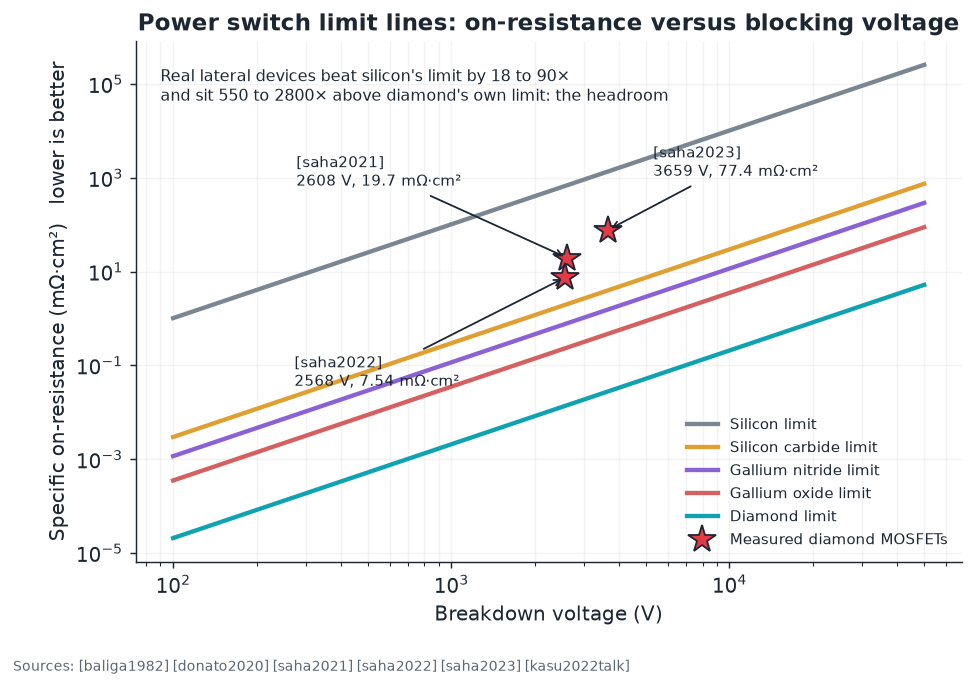
\includegraphics[width=0.8\linewidth]{fig03_ron_vs_bv.png}\end{tikzfigure}
Measured hydrogen-terminated diamond MOSFETs reach \BestBV\,V and beat silicon's limit by \hl{\MeasuredOverSi$\times$}. In an 800\,V electric-vehicle inverter an ideal diamond switch loses \LossDiamond\,W against \LossSiC\,W for silicon carbide. Propagating the published spread of diamond's critical field and hole mobility gives a median advantage of \hl{\UncPowerPfifty$\times$} (P10 to P90: \UncPowerPten{} to \UncPowerPninety$\times$).
\begin{tikzfigure}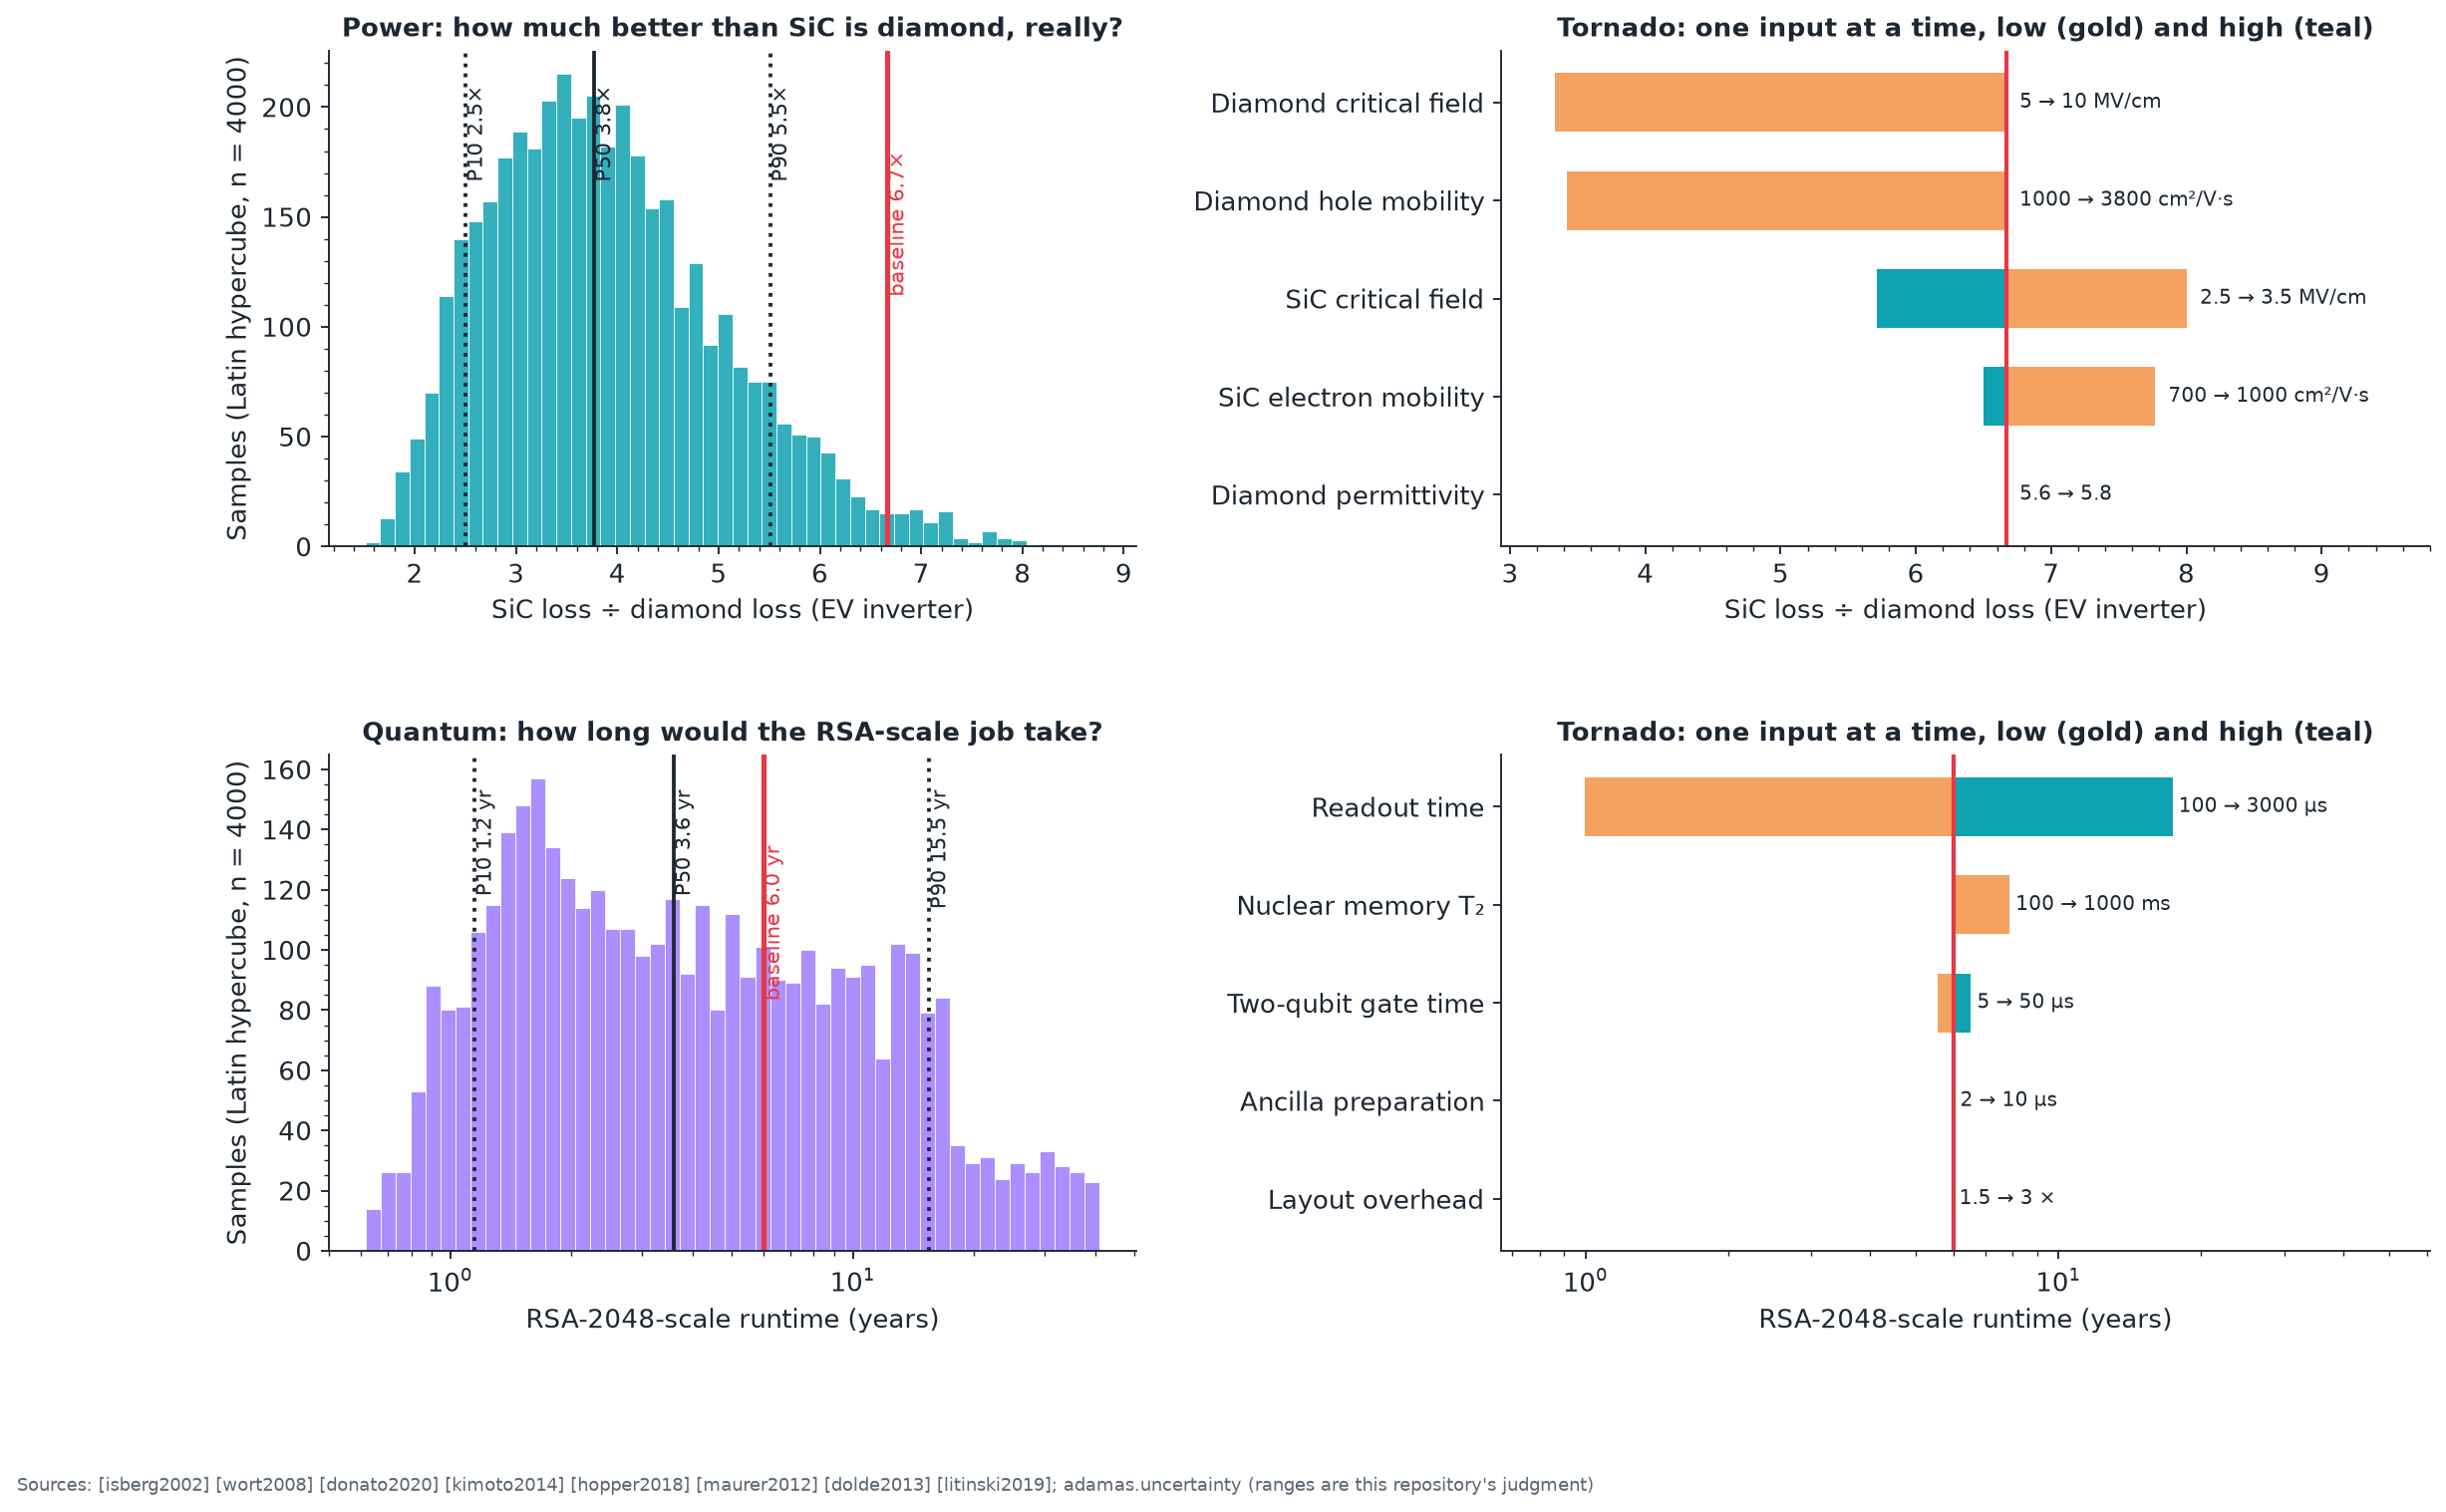
\includegraphics[width=0.95\linewidth]{fig49_uncertainty.png}\end{tikzfigure}}
\block{2 · How to build it}{
\begin{tikzfigure}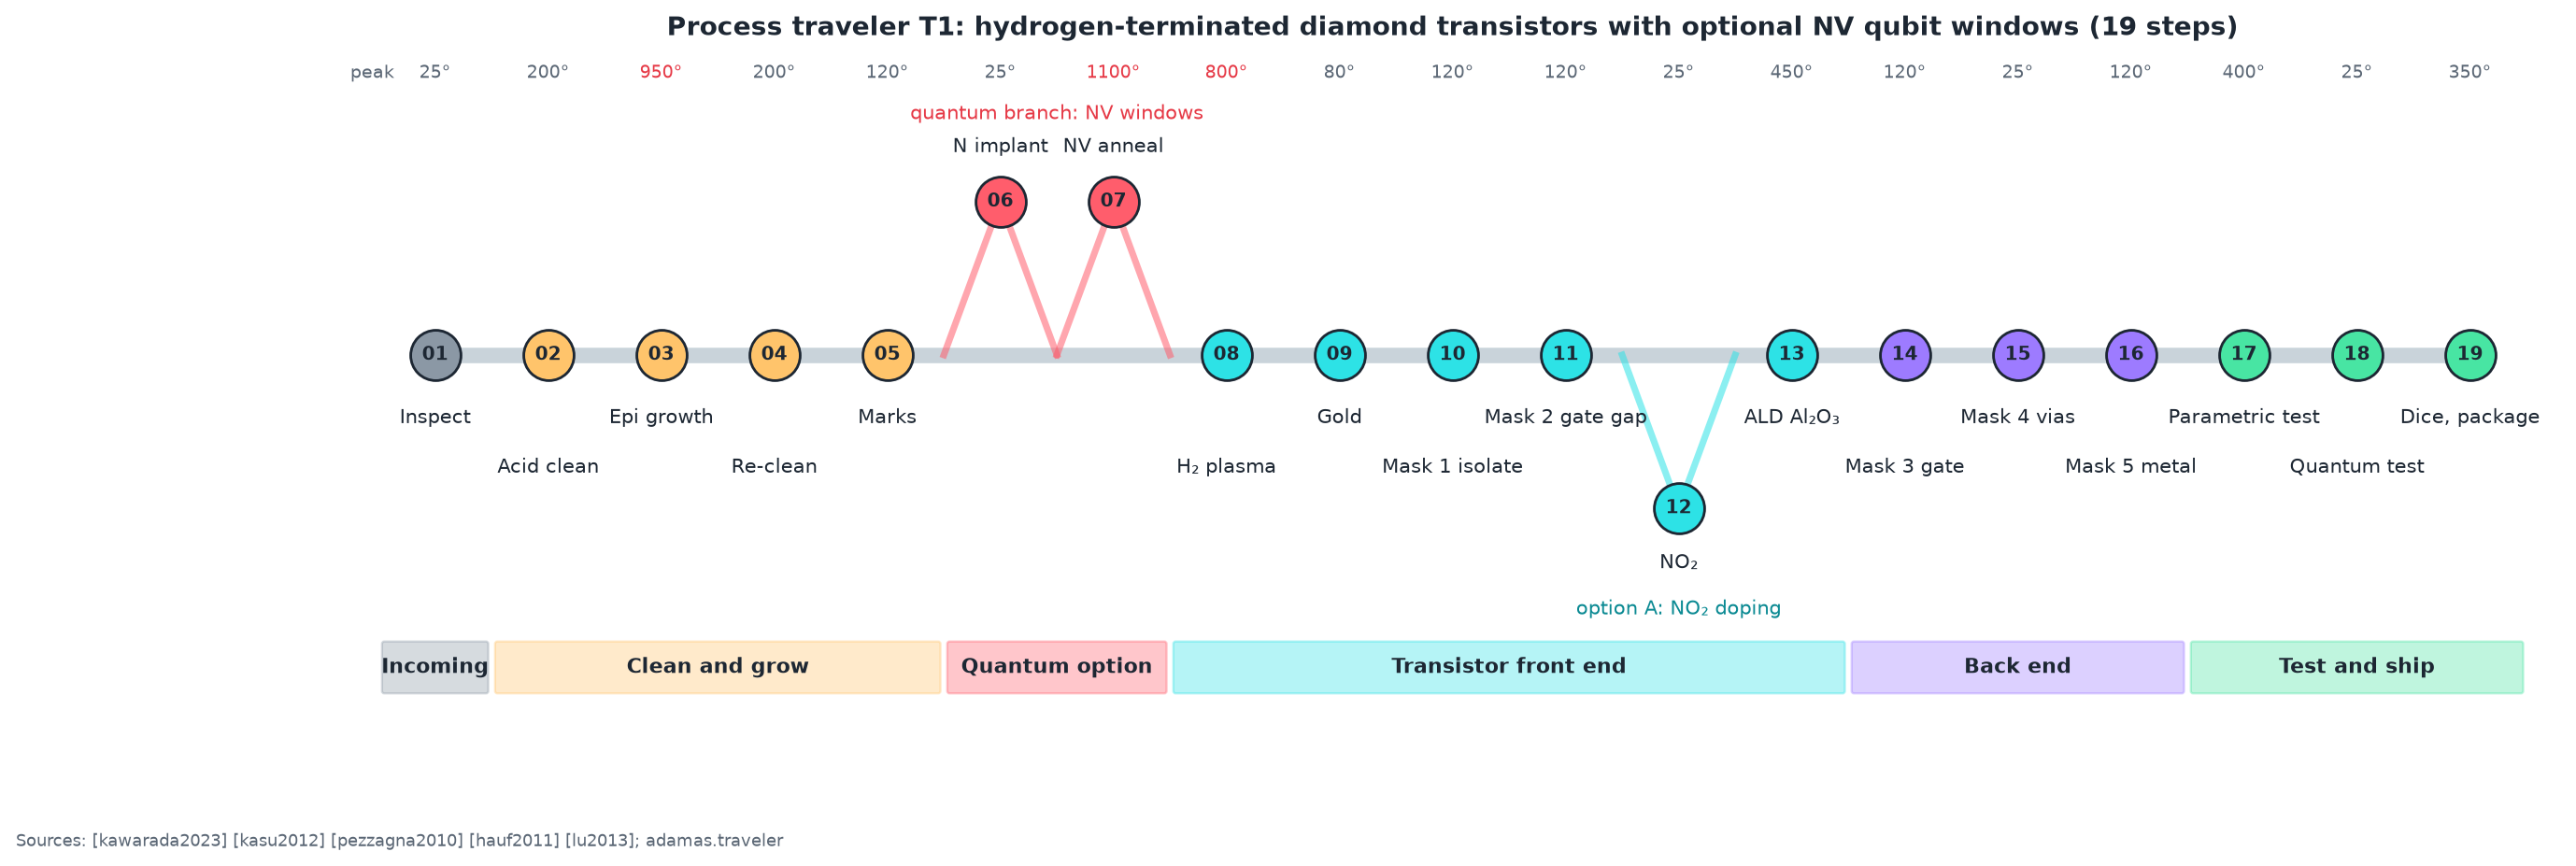
\includegraphics[width=0.95\linewidth]{fig41_process_flow.png}\end{tikzfigure}
A 19-step traveler: hydrogen termination makes the channel, gold protects it, one oxygen plasma isolates devices, and all heat is spent before the first metal. The PDK-0 kit places the 4-bit DIA-4 processor (\DiaCells{} cells) in about 1\,mm$^2$.
}
\block{Validation and reproducibility}{
\begin{minipage}{0.68\linewidth}\ValChecks{} validation checks (\ValPass{} pass) against published results, independent tools, and known answers; \NumVerified{} references verified against Crossref. \texttt{pip install -e ".[dev]" \&\& pytest \&\& make figures paper talk poster} regenerates everything.\end{minipage}\hfill
\begin{minipage}{0.28\linewidth}\centering\qrcode[height=5.5cm]{https://normansrule.github.io/adamas-diamond-framework/}\\\small interactive site\end{minipage}}
\column{0.5}
\block{3 · The qubit bottleneck is preparation}{
\begin{tikzfigure}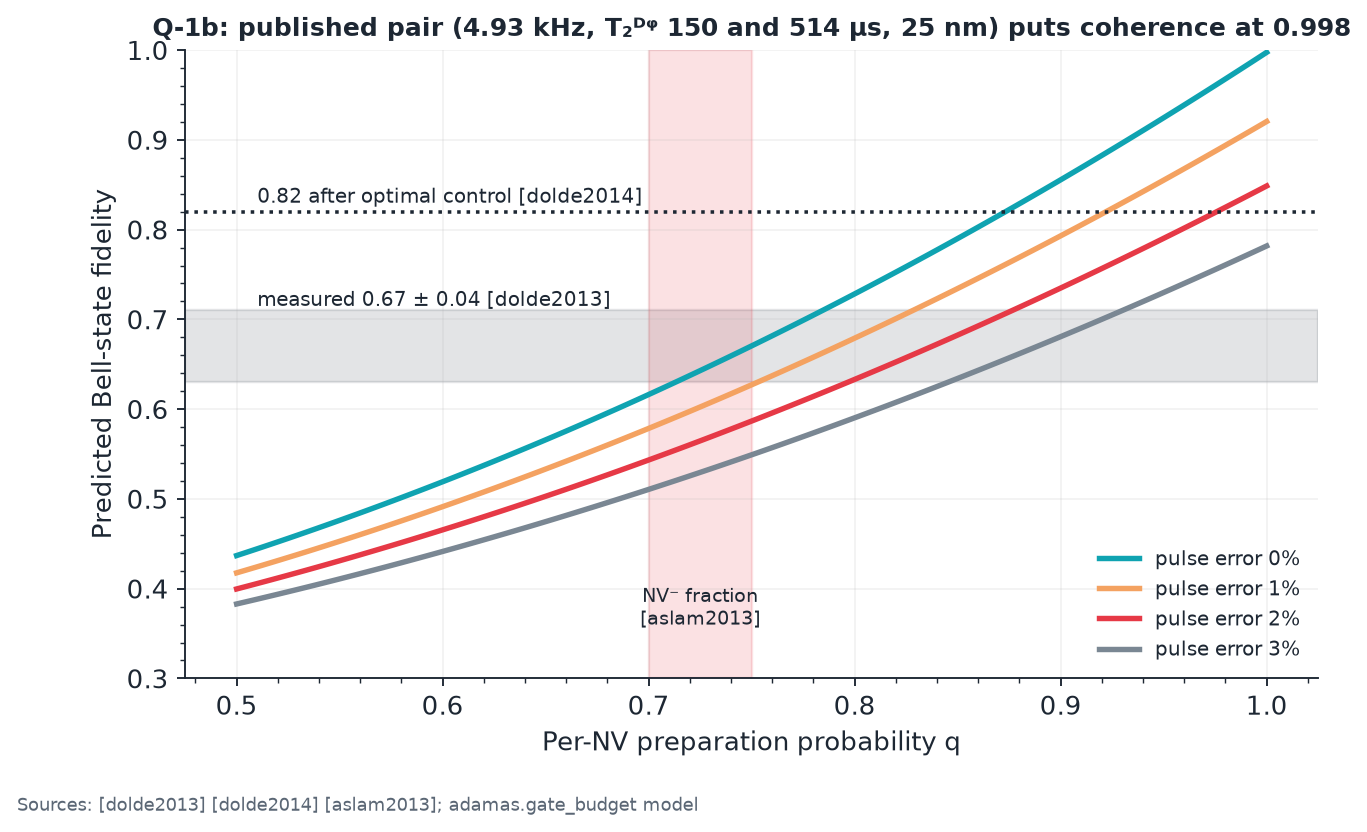
\includegraphics[width=0.95\linewidth]{fig36_published_gate_check.png}\end{tikzfigure}
With the published 25\,nm pair, coherence alone allows a Bell fidelity of \hl{\FcohPublished}; the measured 0.67 means the NV$^-$ charge state was ready only \qForSixtySeven{} of the time.}
\block{4 · Error correction with slow readout}{
\begin{tikzfigure}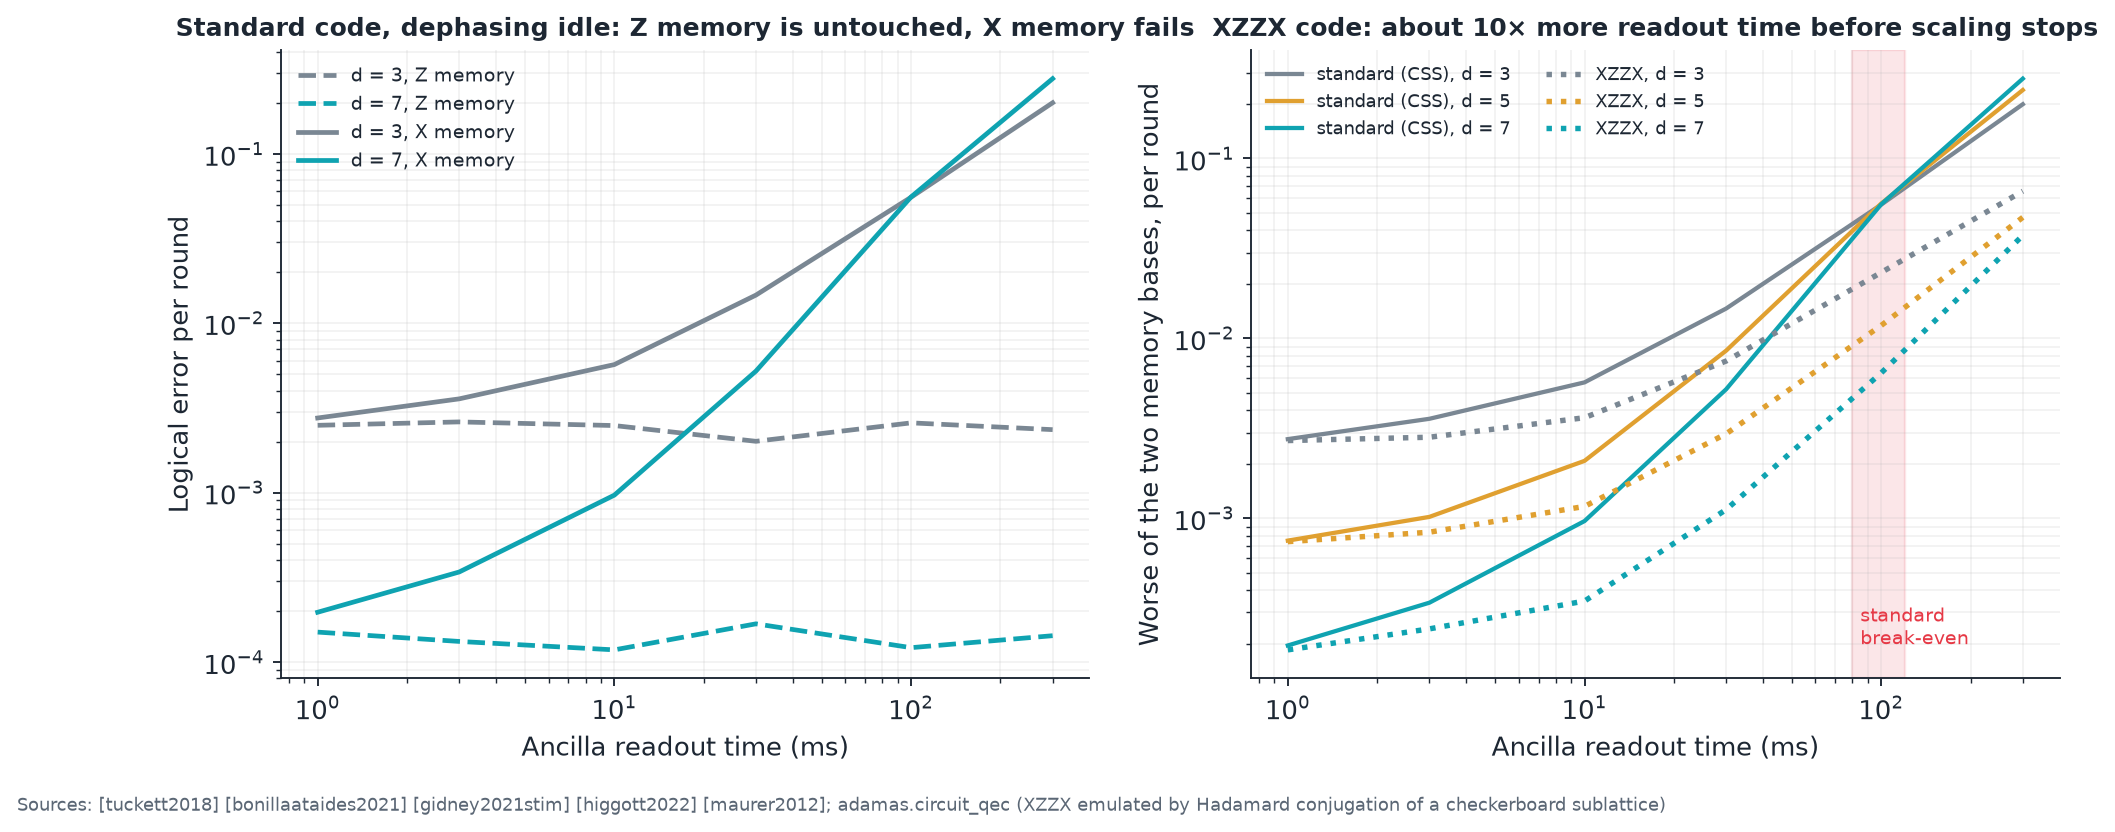
\includegraphics[width=0.95\linewidth]{fig40_biased_noise_xzzx.png}\end{tikzfigure}
Circuit-level simulations (Stim, PyMatching): scaling stops near \BreakevenStdMs\,ms readout for a 1\,s nuclear memory; the bias-tailored XZZX code extends this to about \hl{\BreakevenXZZXMs\,ms}. An RSA-2048-scale machine fits on a \RSADieMm\,mm die but runs \hl{\RSAYears{} years} at 1\,ms readout (P10 to P90: \UncQPten{} to \UncQPninety).}
\block{5 · Try it: experiments from US\$100}{
\begin{tikzfigure}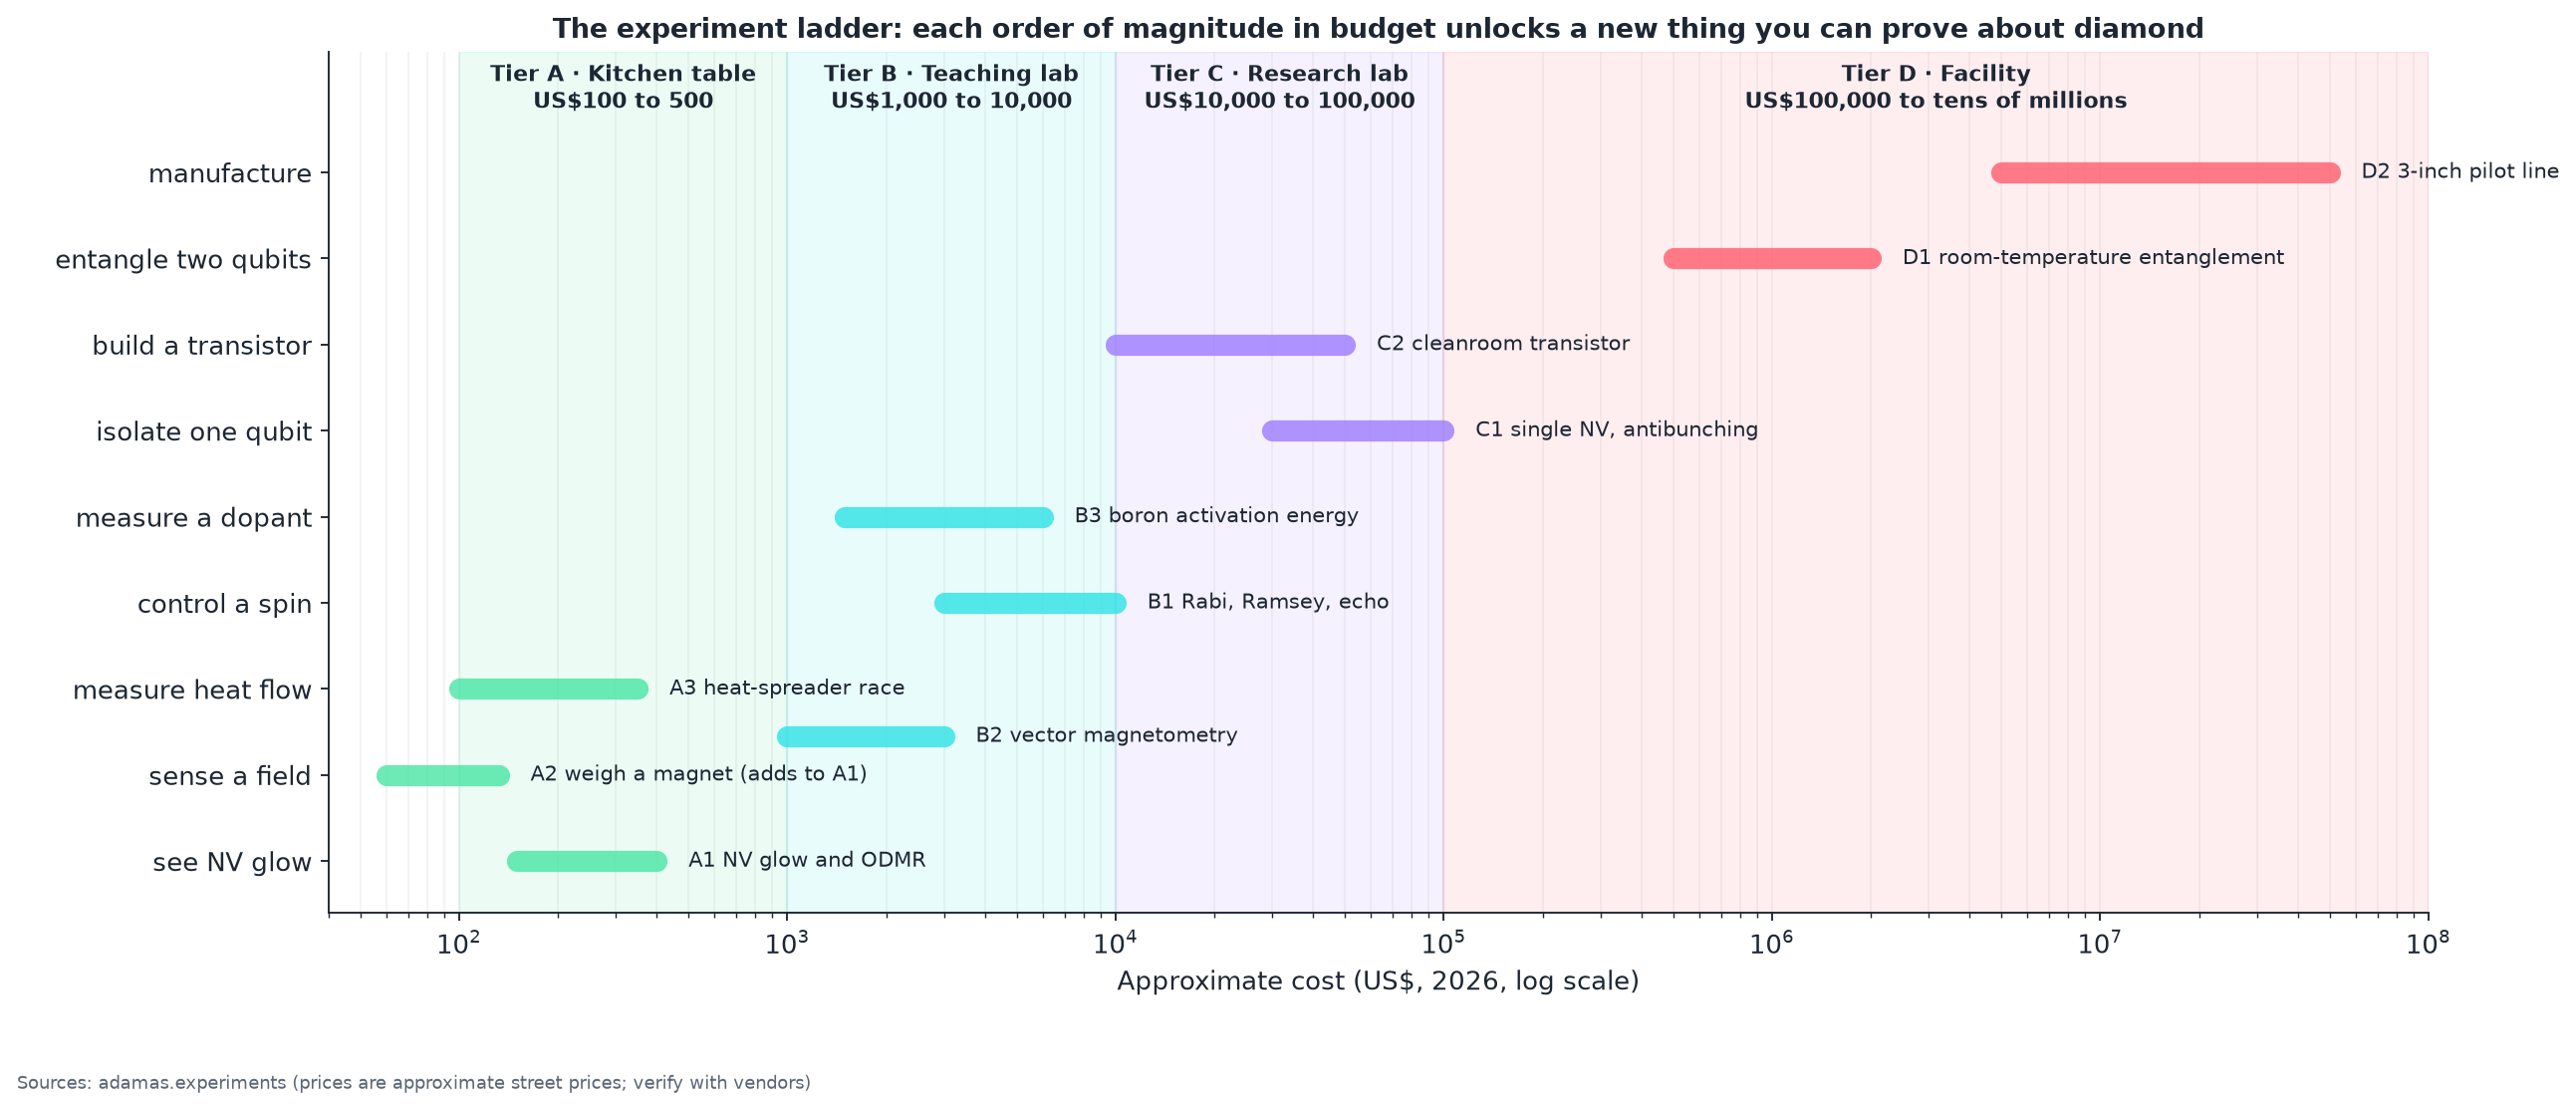
\includegraphics[width=0.95\linewidth]{fig47_experiment_ladder.png}\end{tikzfigure}
Ten experiments in four budgets with parts, steps, safety, and expected results; the A1 ODMR kit ships with Raspberry Pi Pico firmware and a fitter.}
\end{columns}
\end{document}
